\subsection{Giới thiệu}
Những năm gần đây, AI - Artificial Intelligence (Trí Tuệ Nhân Tạo), và cụ thể hơn là Machine Learning (Học Máy hoặc Máy Học) nổi lên như một bằng chứng của cuộc cách mạng công nghiệp lần thứ tư (1 - động cơ hơi nước, 2 - năng lượng điện, 3 - công nghệ thông tin). 
Trí Tuệ Nhân Tạo đang len lỏi vào mọi lĩnh vực trong đời sống mà có thể chúng ta không nhận ra. 
Xe tự hành của Google và Tesla, hệ thống tự tag khuôn mặt trong ảnh của Facebook, trợ lý ảo Siri của Apple, hệ thống gợi ý sản phẩm của Amazon, hệ thống gợi ý phim của Netflix, máy chơi cờ vây AlphaGo của Google DeepMind, …, chỉ là một vài trong vô vàn những ứng dụng của AI/Machine Learning.
\par
Machine Learning là một tập con của AI. 
Theo định nghĩa của Wikipedia, Machine learning is the subfield of computer science that “gives computers the ability to learn without being explicitly programmed”. 
Nói đơn giản, Machine Learning là một lĩnh vực nhỏ của Khoa Học Máy Tính, nó có khả năng tự học hỏi dựa trên dữ liệu đưa vào mà không cần phải được lập trình cụ thể.
\par
Những năm gần đây, khi mà khả năng tính toán của các máy tính được nâng lên một tầm cao mới và lượng dữ liệu khổng lồ được thu thập bởi các hãng công nghệ lớn, Machine Learning đã tiến thêm một bước dài và một lĩnh vực mới được ra đời gọi là Deep Learning (Học Sâu - thực sự tôi không muốn dịch từ này ra tiếng Việt). 
Deep Learning đã giúp máy tính thực thi những việc tưởng chừng như không thể vào 10 năm trước: phân loại cả ngàn vật thể khác nhau trong các bức ảnh, tự tạo chú thích cho ảnh, bắt chước giọng nói và chữ viết của con người, giao tiếp với con người, hay thậm chí cả sáng tác văn hay âm nhạc
\subsection{Phân nhóm các thuật toán}
Theo phương thức học, các thuật toán Machine Learning thường được chia làm 4 nhóm:
\begin{itemize}
\item Supervise learning (học có giám sát)
\item Unsupervised learning ( học không có giám sát)
\item Semi-supervised lerning ( Học bán giám sát)
\item Reinforcement learning ( Học củng cố)
\end{itemize}
\begin{enumerate}
\item \textbf{Học có giám sát (Supervised Learning)}
\par
Supervised learning là thuật toán dự đoán đầu ra (outcome) của một dữ liệu mới (new input) dựa trên các cặp (input, outcome) đã biết từ trước. 
Cặp dữ liệu này còn được gọi là (data, label), tức (dữ liệu, nhãn). 
Supervised learning là nhóm phổ biến nhất trong các thuật toán Machine Learning
\begin{enumerate}
\item \textbf{Classification (Phân loại)}: Một bài toán được gọi là classification nếu các label của input data được chia thành một số hữu hạn nhóm. 
Ví dụ: Gmail xác định xem một email có phải là spam hay không; các hãng tín dụng xác định xem một khách hàng có khả năng thanh toán nợ hay không. 
Ba ví dụ phía trên được chia vào loại này
\par
\item \textbf{Regression (Hồi quy)}
Nếu label không được chia thành các nhóm mà là một giá trị thực cụ thể. Ví dụ: một căn nhà rộng x m2x m2, có yy phòng ngủ và cách trung tâm thành phố z kmz km sẽ có giá là bao nhiêu?
\par
Gần đây Microsoft có một ứng dụng dự đoán giới tính và tuổi dựa trên khuôn mặt. 
Phần dự đoán giới tính có thể coi là thuật toán Classification, phần dự đoán tuổi có thể coi là thuật toán Regression. 
Chú ý rằng phần dự đoán tuổi cũng có thể coi là Classification nếu ta coi tuổi là một số nguyên dương không lớn hơn 150, chúng ta sẽ có 150 class (lớp) khác nhau
\end{enumerate}
\item \textbf{Học không giám sát ( Unsupervise learning)}
\par
Trong thuật toán này, chúng ta không biết được outcome hay nhãn mà chỉ có dữ liệu đầu vào. 
Thuật toán unsupervised learning sẽ dựa vào cấu trúc của dữ liệu để thực hiện một công việc nào đó, ví dụ như phân nhóm (clustering) hoặc giảm số chiều của dữ liệu (dimension reduction) để thuận tiện trong việc lưu trữ và tính toán.
\par
Một cách toán học, Unsupervised learning là khi chúng ta chỉ có dữ liệu vào XX mà không biết nhãn YY tương ứng.
Những thuật toán loại này được gọi là Unsupervised learning vì không giống như Supervised learning, chúng ta không biết câu trả lời chính xác cho mỗi dữ liệu đầu vào. 
Giống như khi ta học, không có thầy cô giáo nào chỉ cho ta biết đó là chữ A hay chữ B. 
Cụm không giám sát được đặt tên theo nghĩa này.
\par
Các bài toán Unsupervised learning được tiếp tục chia nhỏ thành hai loại:
\begin{enumerate}
\item \textbf{Clustering (phân nhóm)}
\par
Một bài toán phân nhóm toàn bộ dữ liệu XX thành các nhóm nhỏ dựa trên sự liên quan giữa các dữ liệu trong mỗi nhóm. 
Ví dụ: phân nhóm khách hàng dựa trên hành vi mua hàng. Điều này cũng giống như việc ta đưa cho một đứa trẻ rất nhiều mảnh ghép với các hình thù và màu sắc khác nhau, ví dụ tam giác, vuông, tròn với màu xanh và đỏ, sau đó yêu cầu trẻ phân chúng thành từng nhóm. 
Mặc dù không cho trẻ biết mảnh nào tương ứng với hình nào hoặc màu nào, nhiều khả năng chúng vẫn có thể phân loại các mảnh ghép theo màu hoặc hình dạng.
\newline
\newline
\item \textbf{Association (kết hợp)}
\par
Là bài toán khi chúng ta muốn khám phá ra một quy luật dựa trên nhiều dữ liệu cho trước. 
Ví dụ: những khách hàng nam mua quần áo thường có xu hướng mua thêm đồng hồ hoặc thắt lưng; những khán giả xem phim Spider Man thường có xu hướng xem thêm phim Bat Man, dựa vào đó tạo ra một hệ thống gợi ý khách hàng (Recommendation System), thúc đẩy nhu cầu mua sắm.
\end{enumerate}
\item \textbf{Học bán giám sát ( Semi-Supervise Learning)}
\par
Các bài toán khi chúng ta có một lượng lớn dữ liệu XX nhưng chỉ một phần trong chúng được gán nhãn được gọi là Semi-Supervised Learning. Những bài toán thuộc nhóm này nằm giữa hai nhóm được nêu bên trên.
\par
Một ví dụ điển hình của nhóm này là chỉ có một phần ảnh hoặc văn bản được gán nhãn (ví dụ bức ảnh về người, động vật hoặc các văn bản khoa học, chính trị) và phần lớn các bức ảnh/văn bản khác chưa được gán nhãn được thu thập từ internet. 
Thực tế cho thấy rất nhiều các bài toán Machine Learning thuộc vào nhóm này vì việc thu thập dữ liệu có nhãn tốn rất nhiều thời gian và có chi phí cao. 
Rất nhiều loại dữ liệu thậm chí cần phải có chuyên gia mới gán nhãn được (ảnh y học chẳng hạn). 
Ngược lại, dữ liệu chưa có nhãn có thể được thu thập với chi phí thấp từ internet.
\newline
\newline   
\item \textbf{Học củng cố ( Reinforcement Learning)}
\par
Reinforcement learning là các bài toán giúp cho một hệ thống tự động xác định hành vi dựa trên hoàn cảnh để đạt được lợi ích cao nhất (maximizing the performance). Hiện tại, Reinforcement learning chủ yếu được áp dụng vào Lý Thuyết Trò Chơi (Game Theory), các thuật toán cần xác định nước đi tiếp theo để đạt được điểm số cao nhất
\begin{figure}[!htbp]
    \centering
    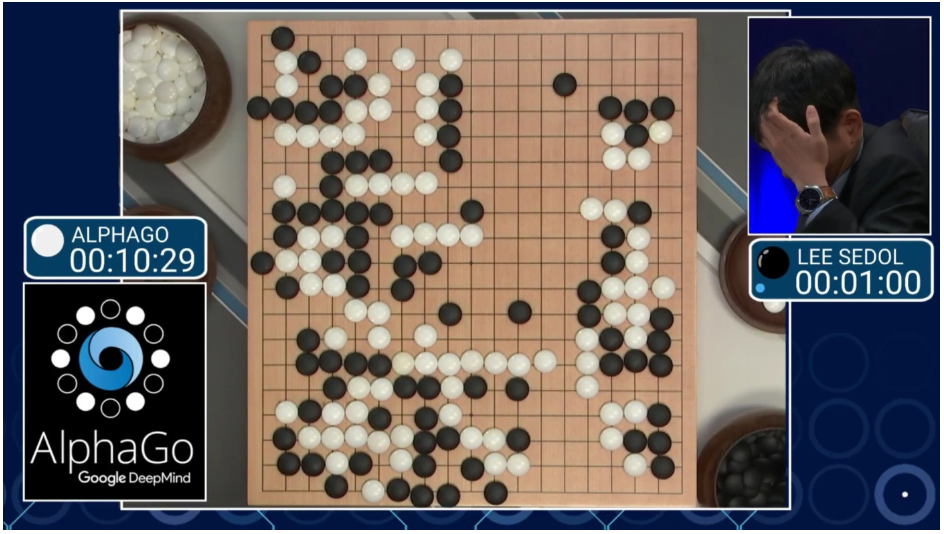
\includegraphics[scale=0.5]{reinforcement_learning}
    \caption{AlphaGo chơi cờ vây với Lee Sedol. AlphaGo là một ví dụ điển hình của Reinforcement Learing}
    \label{fig:x cubed graph}
\end{figure}
\FloatBarrier
\end{enumerate}